\textit{This section was contributed by Bob Myhill}.

This cookbook shows how the ascii data layered plugin for the initial
composition can be used to sample the Crust 1.0 dataset \cite{laske2013update}
at arbitrary resolution.
The dataset itself provides an estimate of the depths of
10 lithological boundaries in the Earth at 1 degree resolution. These layers are:
the top of the mantle, the tops of the lower, middle and upper crust,
the tops of the lower, middle and upper sediments,
the tops of the ice and water layers, and the base of the air (i.e. the topography).
The densities within the layers are assumed to be constant vertically, but vary
laterally.

In this cookbook, we assign the material density from the initial compositional
field defined by Crust 1.0, using a material model plugin based on the \texttt{simpler}
material model. We call this material model ``SimplerWithDensityField''.
The important line in this material model is
\begin{lstlisting}[frame=single,language=C++]
    out.densities[i] = std::max(in.composition[i][density_idx], 1.);
\end{lstlisting}

The plugin can be found at
\url{cookbooks/crust1/plugin/simpler_with_density_field.cc}. Refer to
Section~\ref{sec:plugins} for more information about writing and running
plugins.

The parameter file accompanying this cookbook is located at
\url{cookbooks/crust1/crust1_3d_chunk.prm}. The geometry model used in this
parameter file is a narrow 3D chunk (1 degree wide), which samples the Crust 1.0
dataset through a north-south profile which includes Chomolungma (Mt Everest).
The parts of the parameter file relevant to using the densities from the
Crust 1.0 dataset are as follows:
\begin{itemize}
  \item Load the plugin implementing the new material model:
  \lstinputlisting[language=prmfile]{cookbooks/crust1/doc/crust1_3d_chunk.part1.prm.out}


  \item Read in the Crust 1.0 boundary files:
  \lstinputlisting[language=prmfile]{cookbooks/crust1/doc/crust1_3d_chunk.part2.prm.out}


  \item Declare the correct number of compositional fields:
  \lstinputlisting[language=prmfile]{cookbooks/crust1/doc/crust1_3d_chunk.part3.prm.out}


  \item Declare the parameters for the new material model:
  \lstinputlisting[language=prmfile]{cookbooks/crust1/doc/crust1_3d_chunk.part4.prm.out}

\end{itemize}

The entire parameter file is located in
\url{cookbooks/crust1/crust1_3d_chunk.prm}.


Figure~\ref{fig:crust1} shows the density field and compositional layers
recreated by running the parameter file.

\begin{figure}
  \centering
  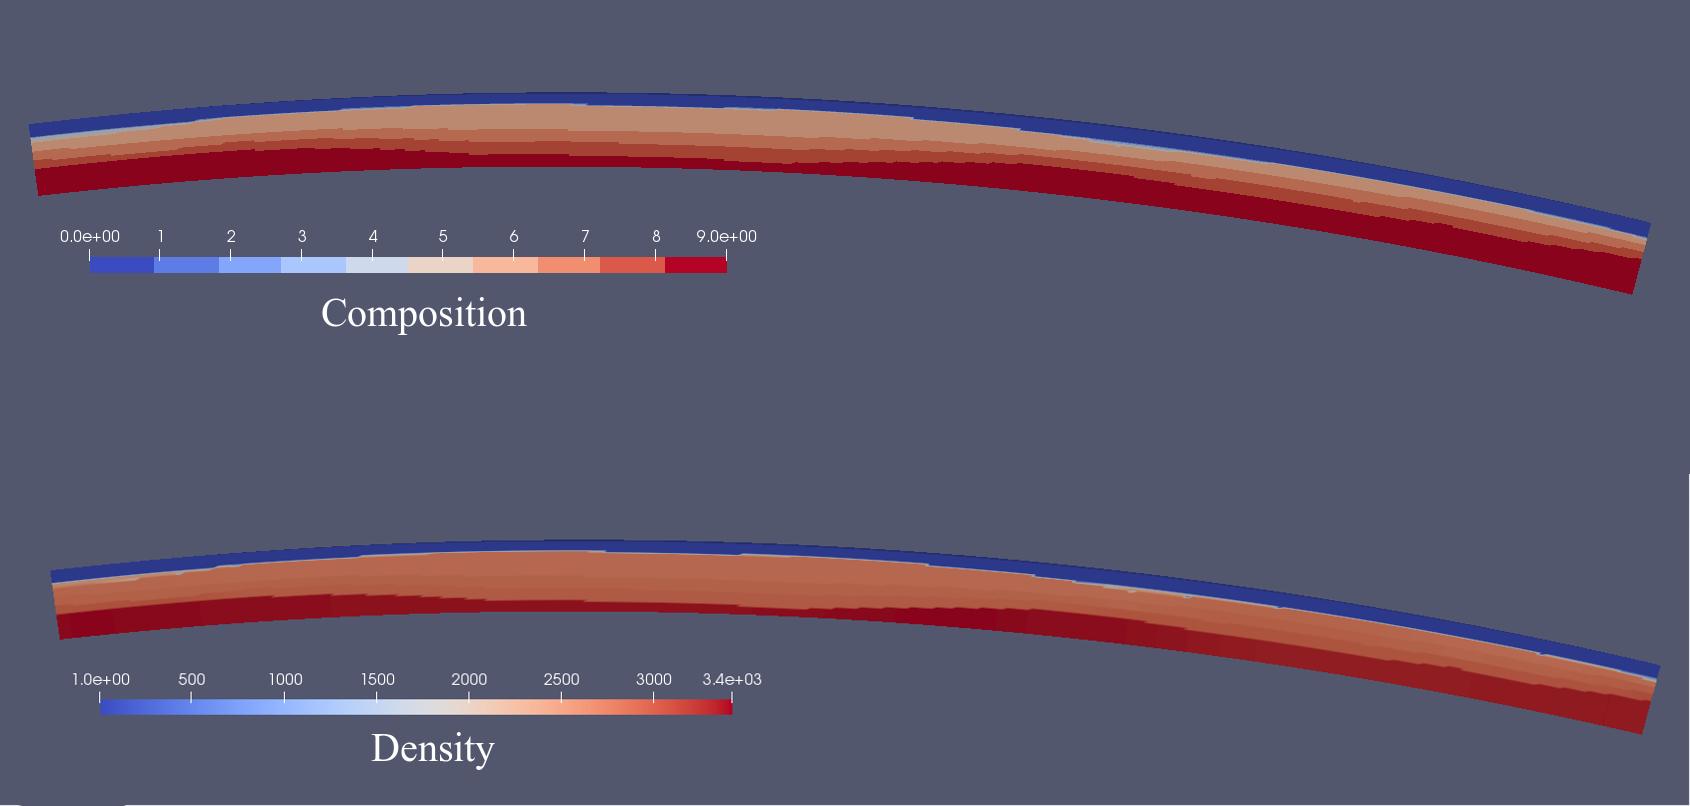
\includegraphics[height=0.25\textwidth]{cookbooks/crust1/doc/crust1_3d_chunk.png}
  \caption{\it A profile through the Crust 1.0 dataset generated using ASPECT's
  ascii data layered plugin for the initial composition. The compositional field
  for the density generated by this plugin is then passed to a simple material model.}
  \label{fig:crust1}
\end{figure}
